\documentclass[letter,11pt]{article}

\usepackage[spanish,es-nodecimaldot]{babel}
\usepackage[utf8]{inputenc}

\usepackage{lmodern}
\usepackage[T1]{fontenc}
\usepackage{textcomp}

\usepackage{framed}
\usepackage[svgnames]{xcolor}
\colorlet{shadecolor}{Gainsboro!50}

\usepackage[labelfont=bf]{caption}
\usepackage{graphicx}
\usepackage{pstricks}

\usepackage{anysize}
\marginsize{3cm}{2cm}{2cm}{3cm}

\usepackage{siunitx}
\usepackage{amsmath}
\usepackage{array}
\usepackage{alltt}

\usepackage{fancyhdr}
\usepackage{lastpage}
\pagestyle{fancy}
\fancyhf{}
\fancyhead[LE,RO]{Laboratorio de Física Básica III}
\fancyfoot[CO,CE]{\thepage\ de \pageref{LastPage}}

\special{papersize=215.9mm,279.4mm}

\usepackage[
    pdfauthor={
        Bastos Lizondo Rosemary;
        Blanco Alconz John Brandon;
        Caballero Burgoa Carlos Eduardo;
        Villena Gutiérrez Ismael Cristian
    },%
    pdftitle={Laboratorio de Física Básica III},%
    pdfsubject={Ley de Coulomb},%
    colorlinks,%
    citecolor=black,%
    filecolor=black,%
    linkcolor=black,%
    urlcolor=black,
    breaklinks]{hyperref}
\usepackage{breakurl}

\newcommand{\blankpage}{
\newpage
\thispagestyle{empty}
\mbox{}
\newpage
}

\renewcommand{\arraystretch}{1.2}

\begin{document}

\begin{titlepage}
\begin{center}
{\Large UNIVERSIDAD MAYOR DE SAN SIMÓN}\\
\vspace*{0.15cm}
{\large FACULTAD DE CIENCIAS Y TECNOLOGÍA}\\
\vspace*{0.10cm}
DEPARTAMENTO DE FÍSICA\\
\vspace*{3.0cm}
{\Large \textbf{LABORATORIO DE FÍSICA BÁSICA III}}\\
\vspace*{0.3cm}
{\Large \textbf{INFORME No. 1}}\\
\vspace*{3.5cm}
{\Large \textbf{LEY DE \emph{COULOMB}}}\\
\end{center}

\vspace*{6.2cm}
\leftskip=7.95cm
\noindent
\textbf{Integrantes:}\\
Bastos Lizondo Rosemary.\\
Blanco Alconz John Brandon.\\
Caballero Burgoa Carlos Eduardo.\\
Villena Gutiérrez Ismael Cristian.\\
\newline
\textbf{Docente:}\\
Ing. Flores Flores, Freddy.\\
\newline
\textbf{Grupo:} G3.\\
\textbf{Fecha de entrega:} 20 de Marzo del 2021.\\

\end{titlepage}

\section{Evaluación previa}
\begin{enumerate}
\item \textbf{¿A qué llamamos ley de \emph{Coulomb}?} \\
La ley de \emph{Coulomb} también conocida como ley de cargas, tiene que ver con
las cargas eléctricas de un material, es decir, depende de si sus cargas son 
negativas o positivas.

Puede puede expresarse como: ``La magnitud de cada una de las fuerzas eléctricas
con las que interactúan dos cargas puntuales en reposo es directamente
proporcional al producto de la magnitud de ambas cargas e inversamente
proporcional al cuadrado de la distancia que las separa y tiene la dirección de
la línea que las une. La fuerza es de repulsión si las cargas son de igual
signo, y de atracción si son de signo contrario''.
\item \textbf{¿Qué es la permitividad del vacío y qué unidades tiene?} \\
La permitividad de vacío, comúnmente denominada $\varepsilon_0$ es el valor de
la permitividad dieléctrica absoluta del vacío clásico. Alternativamente, puede
denominarse permitividad del espacio libre, constante eléctrica o capacitancia
distribuida del vacío. Es una constante física ideal (línea de base). La unidad
de medida en el Sistema Internacional es el faradio por metro ($F/m$).
\item \textbf{¿Qué es la capacitancia?} \\
La capacitancia es la capacidad de un componente o circuito para recoger y
almacenar energía en forma de carga eléctrica.

Los capacitores son dispositivos que almacenan energía, disponibles en muchos
tamaños y formas. Consisten en dos placas de material conductor, generalmente un
metal fino ubicado entre un aislador de cerámica, película, vidrio u otros
materiales, incluso aire.
\item \textbf{¿A qué llamamos corrientes de fuga y cuando ocurre?} \\
En toda instalación eléctrica por el conductor de protección circula corriente a
tierra, esta misma tiene por nombre corriente de fuga. Ocurre cuando el
aislamiento del conductor está deteriorado, envejecido o tiene algún mal sello,
al ocurrir esto corre el riesgo de que el conductor haga contacto con otro cuerpo
conductor.
\item \textbf{¿Qué cuidados se debe tener para que no ocurra ``\emph{leakage
currents}'' o corrientes de fuga?} \\
Cuantificar la corriente de fuga, identificar su origen, esto se puede hacer
mediante una pinza amperimétrica para medidas de corrientes de carga.
\item \textbf{Mencione cuales creen que son los cuidados que se deben tener con
el manejo de fuentes de alta tensión?} \\
Antes de iniciar cualquier trabajo eléctrico sin tensión debemos desconectar
todas las posibles alimentaciones a la línea. Puesta a tierra, en el caso de que
la línea o el equipo volviesen a ponerse en tensión, bien por una
realimentación, o descarga, rayo, se produciría un cortocircuito y se derivaría
la corriente de tierra, quedando sin peligro la parte afectada por los trabajos.
Realizar inspecciones periódicas de las instalaciones.
\end{enumerate}

\section{Objetivos}
\begin{itemize}
\item Verificar la ley de \emph{Coulomb} determinando la relación de la fuerza
    como función de la distancia entre dos esferas cargadas igualmente.
\item Estimar el valor de la permitividad del vacío $\varepsilon_0$.
\end{itemize}

\section{Fundamento teórico}

La ley de \emph{Coulomb} llamado así en honor al físico francés \emph{Charles A.
Coulomb} quién demostró la siguiente relación:

\begin{equation}
    F = \frac{1}{4 \pi \varepsilon_0} \frac{| Q_1 Q_2 |}{d^2}
\label{coulomb}
\end{equation}

Esta ley enuncia que: ''la fuerza eléctrica que ejercen entre sí, dos cargas
puntuales en reposo, es directamente proporcional al producto de sus cargas, e
inversamente proporcional al cuadrado de la distancia que los separa. Tal fuerza
se aplica en los respectivos centros de las cargas y están dirigidas a lo largo
de la línea que las une. La fuerza es de repulsión si las cargas son de igual
signo, y de atracción si son de signo contrario'' véase
\textbf{Figura \ref{figura1}}.

\begin{figure}[!h]
\centering
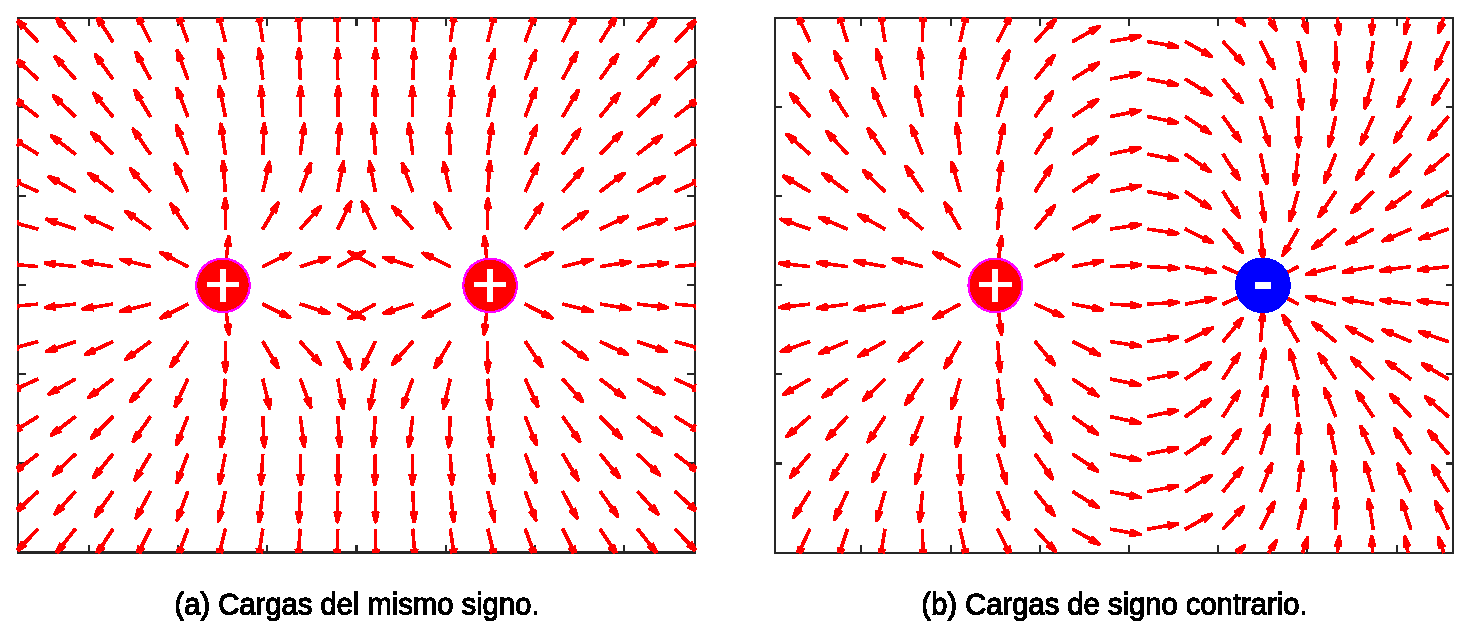
\includegraphics[scale=0.58]{resources/figura1.eps}
\caption{Comportamiento de la intensidad del campo eléctrico entre cargas
puntuales.}
\label{figura1}
\end{figure}

\section{Materiales}
\begin{itemize}
\item Simulador «PhET Interactive Simulations» Ley de \emph{Coulomb} (Escala
macro).
\end{itemize}

\section{Procedimiento experimental}
A continuación se describe el procedimiento experimental que se llevará a
cabo.

\begin{enumerate}
\item Ir al simulador ubicado en la dirección web:
(https://phet.colorado.edu/sims/html/coulombs-law/latest/coulombs-law\_es.html),
tal como se muestra en la \textbf{Figura \ref{figura2}}.
\begin{figure}[!h]
\centering
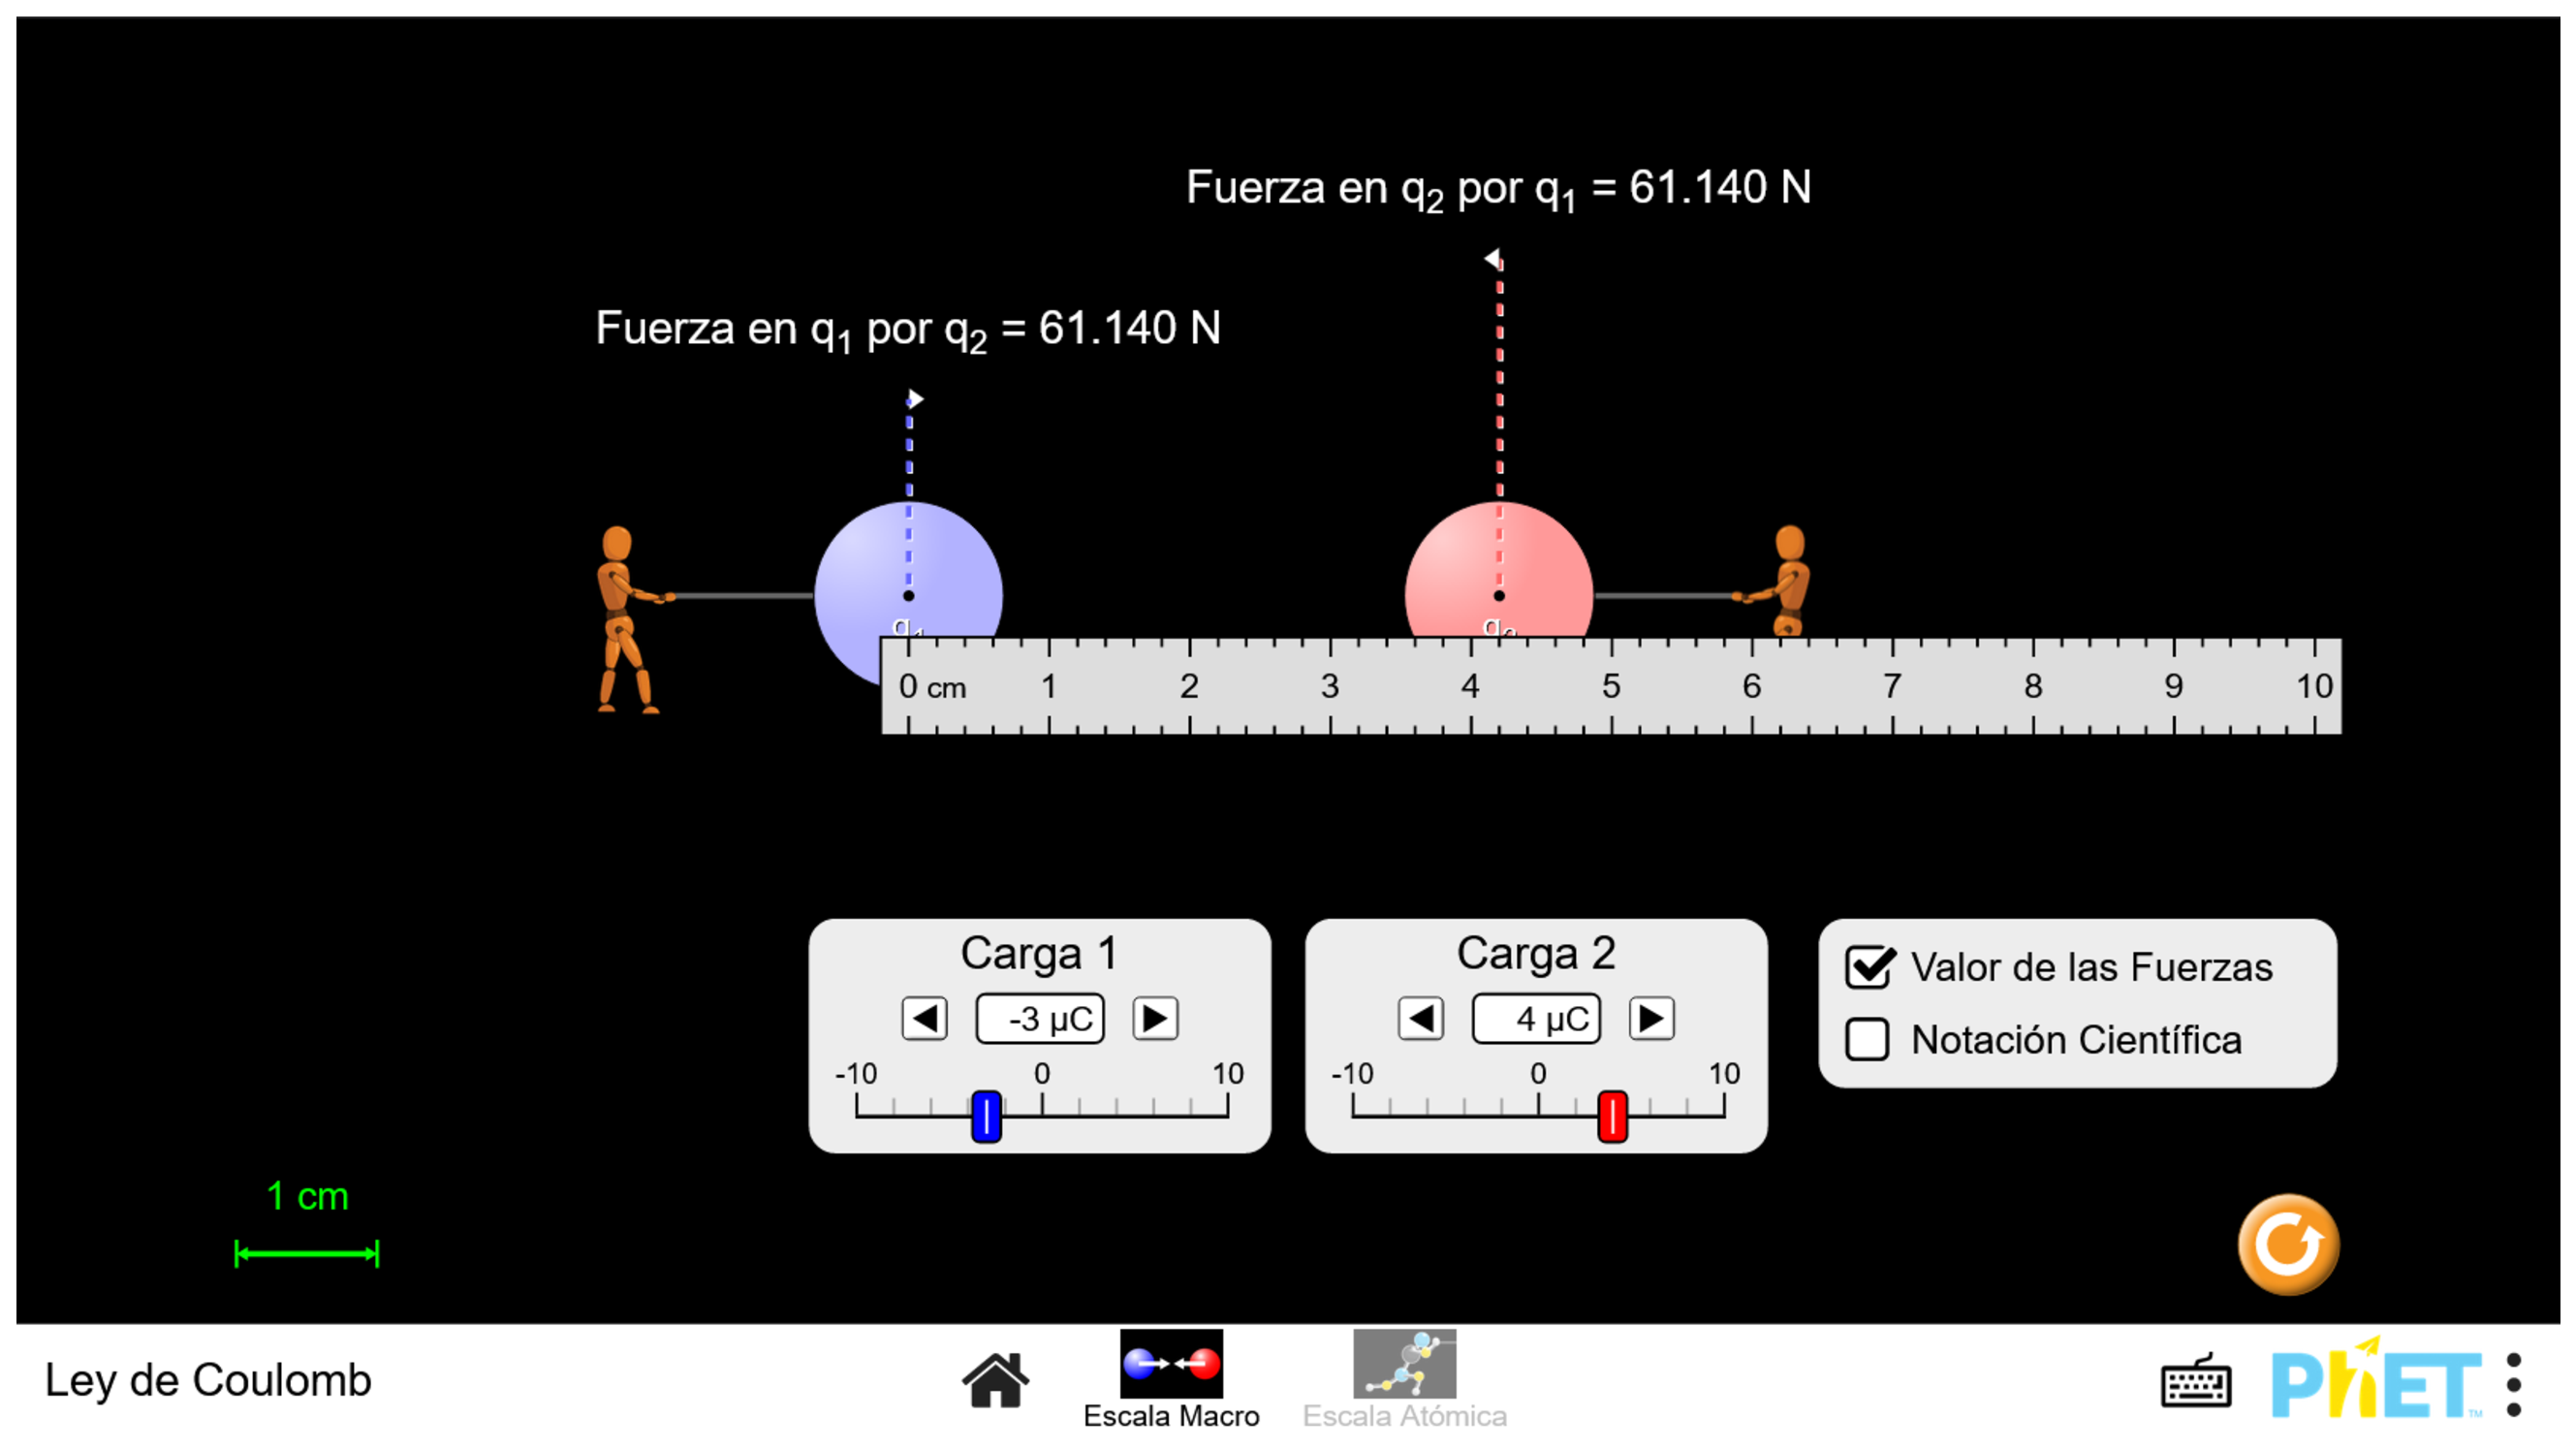
\includegraphics[scale=0.30]{resources/figura2.eps}
\caption{Simulador para la ley de \emph{Coulomb}.}
\label{figura2}
\end{figure}
\item Establecer las cargas fijas $Q_1$ y $Q_2$.
\item Se procede a elegir una distancia entre las cargas $Q_1$ y $Q_2$ y tomar
su respectivo valor de fuerza, tomando 8 datos.
\item Registrar las mediciones tomadas, elaborar las gráficas e interpretar los
resultados.
\end{enumerate}

\section{Resultados}

Carga escogida para la esfera 1:

\begin{equation*}
    Q_1 = -3 \mu C
\end{equation*}

Carga escogida para la esfera 2:

\begin{equation*}
    Q_2 = 4 \mu C
\end{equation*}

En el \textbf{Cuadro \ref{cuadro1}} se presentan los valores de la fuerza
eléctrica ($F$) para diferentes valores de distancia ($d$).

\begin{table}[!h]
\begin{center}
\begin{tabular}{|c|>{\centering}m{3.0cm}<{\centering}
                  |>{\centering}m{3.0cm}<{\centering}|}
\hline
\multicolumn{3}{|c|}{Precisión del instrumento: 0.2[cm]} \\
\hline
$i$ & $d_i [cm]$ & $F_i [N]$ \tabularnewline \hline
1 & 1.4 & 550.258 \tabularnewline \hline
2 & 2.0 & 269.627 \tabularnewline \hline
3 & 3.0 & 119.834 \tabularnewline \hline
4 & 4.2 &  61.140 \tabularnewline \hline
5 & 5.0 &  43.140 \tabularnewline \hline
6 & 5.6 &  34.391 \tabularnewline \hline
7 & 6.4 &  26.331 \tabularnewline \hline
8 & 7.8 &  17.727 \tabularnewline \hline
\end{tabular}
\caption{Mediciones de fuerza y distancia.}
\label{cuadro1}
\end{center}
\end{table}

A partir de los datos del \textbf{Cuadro \ref{cuadro1}}, se obtiene la gráfica
presentada en la \textbf{Figura \ref{figura3}}.

\begin{figure}[!h]
\centering
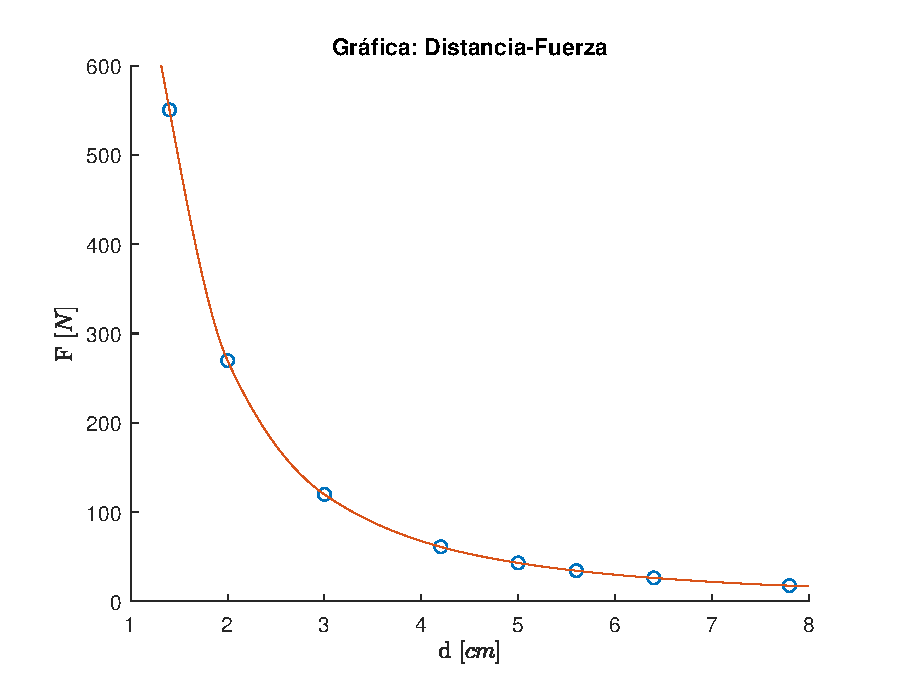
\includegraphics[scale=1.0]{resources/p1.eps}
\caption{Gráfica de fuerza eléctrica en función de la distancia.}
\label{figura3}
\end{figure}

Por la forma de la \textbf{Figura \ref{figura3}} el modelo que se asume para la
relación funcional es:

\begin{equation*}
    F = a d^b
\end{equation*}

Aplicando logaritmos a ambos lados de la ecuación obtenemos:

\begin{equation*}
    \log F = \log a + b \log d
\end{equation*}

Haciendo los siguientes cambios de variables:

\begin{equation*}
    F' = \log F
\end{equation*}
\begin{equation*}
    A = \log a
\end{equation*}
\begin{equation*}
    B = b
\end{equation*}
\begin{equation*}
    d' = \log d
\end{equation*}

Se obtiene:

\begin{equation*}
    F' = A + B d'
\end{equation*}

En el \textbf{Cuadro \ref{cuadro2}} pueden apreciarse los valores de la función
aplicando logaritmos, tales datos generan la gráfica presentada en la
\textbf{Figura \ref{figura4}}.

\begin{table}[!h]
\begin{center}
\begin{tabular}{|c|>{\centering}m{3.0cm}<{\centering}
                  |>{\centering}m{3.0cm}<{\centering}|}
\hline
$i$ & $d'_i$ & $F'_i$ \tabularnewline \hline
1 & 0.1461 & 2.7406 \tabularnewline \hline
2 & 0.3010 & 2.4308 \tabularnewline \hline
3 & 0.4771 & 2.0786 \tabularnewline \hline
4 & 0.6232 & 1.7863 \tabularnewline \hline
5 & 0.6990 & 1.6349 \tabularnewline \hline
6 & 0.7482 & 1.5364 \tabularnewline \hline
7 & 0.8062 & 1.4205 \tabularnewline \hline
8 & 0.8921 & 1.2486 \tabularnewline \hline
\end{tabular}
\caption{Valores logaritmizados.}
\label{cuadro2}
\end{center}
\end{table}

\begin{figure}[!h]
\centering
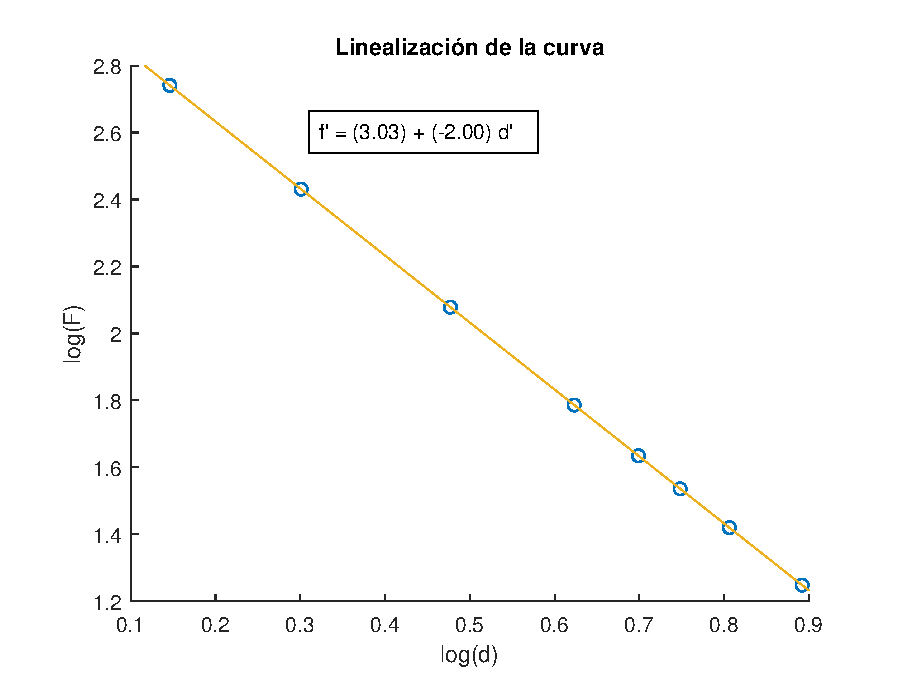
\includegraphics[scale=1.0]{resources/p2.eps}
\caption{Gráfica de la función linealizada.}
\label{figura4}
\end{figure}

Calculamos los parámetros de la recta por el método de los mínimos cuadrados,
con la ayuda de los datos presentados en el \textbf{Cuadro \ref{cuadro3}}.

\begin{table}[!h]
\begin{center}
\begin{tabular}{|c|>{\centering}m{1.4cm}<{\centering}
                  |>{\centering}m{1.4cm}<{\centering}
                  |>{\centering}m{1.4cm}<{\centering}
                  |>{\centering}m{1.4cm}<{\centering}
                  |>{\centering}m{3.2cm}<{\centering}
                  |>{\centering}m{3.2cm}<{\centering}|}
\hline
$i$ & $d'_i F'_i$ & $d'^2_i$ & $F'^2_i$ & $Y$ & $\delta_i$ & $\delta^2_i$ \tabularnewline \hline
1 & 0.4005 & 0.0214 & 7.5107 & 2.7406 & \num{ 0.0183e-5} & \num{0.0003e-10} \tabularnewline \hline
2 & 0.7317 & 0.0906 & 5.9086 & 2.4308 & \num{ 0.0805e-5} & \num{0.0065e-10} \tabularnewline \hline
3 & 0.9917 & 0.2276 & 4.3205 & 2.0786 & \num{-0.0357e-5} & \num{0.0013e-10} \tabularnewline \hline
4 & 1.1133 & 0.3884 & 3.1910 & 1.7863 & \num{ 0.0798e-5} & \num{0.0064e-10} \tabularnewline \hline
5 & 1.1427 & 0.4886 & 2.6728 & 1.6349 & \num{-0.3221e-5} & \num{0.1037e-10} \tabularnewline \hline
6 & 1.1495 & 0.5598 & 2.3607 & 1.5364 & \num{-0.2612e-5} & \num{0.0682e-10} \tabularnewline \hline
7 & 1.1452 & 0.6499 & 2.0177 & 1.4205 & \num{ 0.3714e-5} & \num{0.1379e-10} \tabularnewline \hline
8 & 1.1139 & 0.7958 & 1.5591 & 1.2486 & \num{ 0.0689e-5} & \num{0.0048e-10} \tabularnewline \hline
\end{tabular}
\caption{Valores para el método de mínimos cuadrados.}
\label{cuadro3}
\end{center}
\end{table}

\begin{equation*}
    n = 8
\end{equation*}
\begin{equation*}
    \sum d'_i = 4.6930
\end{equation*}
\begin{equation*}
    \sum F'_i = 14.8767
\end{equation*}
\begin{equation*}
    \sum d'^2_i = 3.2222
\end{equation*}
\begin{equation*}
    \sum F'^2_i = 29.5411
\end{equation*}
\begin{equation*}
    \sum d'_i F'_i = 7.7886
\end{equation*}
\begin{equation*}
    \Delta_1 = n \sum d'^2_i - \left( \sum d'_i \right)^2 = 3.7534
\end{equation*}
\begin{equation*}
    \Delta_2 = n \sum F'^2_i - \left( \sum F'_i \right)^2 = 15.0136
\end{equation*}
\begin{equation*}
    A = \frac{\sum F'_i \sum d'^2_i - \sum d'_i F'_i \sum d'_i}{\Delta_1} = 3.0328
\end{equation*}
\begin{equation*}
    B = \frac{n \sum d'_i F'_i - \sum d'_i \sum F'_i}{\Delta_1} = -2.0000
\end{equation*}
\begin{equation*}
    \sum \delta^2 = \num{3.2909e-11}
\end{equation*}
\begin{equation*}
    \sigma^2 = \frac{\sum \delta^2_i}{n-2} = \num{5.4849e-12}
\end{equation*}
\begin{equation*}
    \sigma_A = \sqrt{\frac{\sigma^2 \sum d^2_i}{\Delta_1}} = \num{2.1699e-6}
\end{equation*}
\begin{equation*}
    \sigma_B = \sqrt{\frac{\sigma^2 n}{\Delta_1}} = \num{3.4191e-6}
\end{equation*}

\begin{equation*}
    A = (3.03 \pm \num{2.2e-6})[u]; \num{7.1e-5}\%
\end{equation*}
\begin{equation*}
    B = (-2.0 \pm \num{3.4e-6})[u]; \num{1.7e-4}\%
\end{equation*}

Siendo el coeficiente de correlación:

\begin{equation*}
    R = \frac{n \sum d'_i F'_i - (\sum d'_i)(\sum F'_i)}{\sqrt{\Delta_1 \Delta_2}} = -1.0000
\end{equation*}

\textbf{Debido a que estamos trabajando en un simulador ideal, podemos verificar
que los resultados para los errores son próximos a cero y el coeficiente de
correlación igual a -1.}
\\

La ecuación de la recta resultante es:

\begin{equation*}
    F' = 3.03 - 2.0 d'
\end{equation*}

A partir de los parámetros de recta $A$ y $B$, calculamos los parámetros $a$ y
$b$ de la curva original y sus errores por el método de propagación de errores:

\begin{equation*}
    a = antilog(A) = antilog(3.03) = 1078.5
\end{equation*}
\begin{equation*}
    b = B = 2.0
\end{equation*}
\begin{equation*}
    e_a = 10^A ln(10) e_A = 10^{(3.03)} ln(10) \num{2.17e-6} = \num{5.4e-3}
\end{equation*}
\begin{equation*}
    e_b = e_B = \num{3.4e-6}
\end{equation*}

Obteniendo finalmente los valores de la curva:

\begin{equation*}
    a = (1078.5 \pm \num{5.4e-3})[cm^2 N]; \num{5e-4}\%
\end{equation*}
\begin{equation*}
    b = (-2.0 \pm \num{3.4e-6})[u]; \num{1.7e-4}\%
\end{equation*}

La ecuación de la curva resultante es:

\begin{equation}
    F = a d^b = 1078.5 d^{-2} = \frac{1078.5}{d^2}
\label{curva}
\end{equation}

Comprobándose la relación entre la Fuerza y la distancia señalada por la ley de
\emph{Coulomb}.

\begin{center}
\begin{tabular}{|>{\centering}m{9.2cm}<{\centering}|}
\hline
\textbf{Resultado} 
\tabularnewline \hline
\\
\Large{$F \propto \frac{1}{d^2}$} \tabularnewline
\\
\hline
\end{tabular}
\end{center}

Se determinará el valor de la permitividad del vacío, igualando la ecuación
(\ref{coulomb}) y la ecuación (\ref{curva}):

\begin{equation*}
    \frac{1}{4 \pi \varepsilon_0} \frac{| Q_1 Q_2 |}{d^2} = \frac{a}{d^2}
\end{equation*}

Y despejando $\varepsilon_0$ obtenemos:

\begin{equation}
    \varepsilon_0 = \frac{| Q_1 Q_2 |}{4 \pi a}
\end{equation}

Calculando el valor representativo:

\begin{equation*}
    \varepsilon_0 = \frac{|(-3)(4)|}{4 \pi (1078.5)} = \num{8.8e-4}
\end{equation*}

La derivada parcial es:

\begin{equation*}
    \frac{\partial{\varepsilon_0}}{\partial{a}} = -\frac{|Q_1 Q_2|}{4 \pi a^2}
\end{equation*}

Siendo el error de la medición:

\begin{equation}
    e_\varepsilon = \frac{|Q_1 Q_2|}{4 \pi a^2} e_a = \num{4.4e-9}
\end{equation}

Resultando la medición:

\begin{equation*}
    \varepsilon_0 = (\num{8.8e-4} \pm \num{4.4e-9}) [\mu C^2/cm^2 N]; \num{5e-4} \%
\end{equation*}

Convirtiendo el resultado hallado de la permitividad del vacío a unidades del
sistema internacional (SI), obtenemos:

\begin{center}
\begin{tabular}{|>{\centering}m{11.0cm}<{\centering}|}
\hline
\textbf{Resultado}
\tabularnewline \hline
\\
$\varepsilon_0 = (\num{8.8542e-12} \pm \num{4.424e-17}) [C^2/m^2 N]; \num{5e-4} \%$ \tabularnewline
\\
\hline
\end{tabular}
\end{center}

\section{Cuestionario}

\begin{enumerate}
\item \textbf{Calcular la diferencia porcentual entre el valor de
$\varepsilon_0$ experimental con el valor teórico.}

Siendo la constante teórica de permitividad del vacío:

\begin{equation*}
    \varepsilon_t = \num{8.8541878176e-12} [C^2/m^2 N]
\end{equation*}

Obtenemos una diferencia porcentual de:

\begin{equation}
    \left(\frac{|\varepsilon_0 - \varepsilon_t|}{\varepsilon_t}\right) \times 100 = 0.00016 \%
\end{equation}

\item \textbf{\emph{Charles A. Coulomb} demostró la existencia de la fuerza
eléctrica con una balanza de torsión, explique el principio de la balanza de
torsión.}

La balanza de torsión (véase \textbf{Figura \ref{figura5}}) consiste en dos
bolas de metal sujetas por los dos extremos de una barra suspendida por un
cable, filamento o chapa delgada. Para medir la fuerza electrostática se puede
poner una tercera bola cargada a una cierta distancia. Las dos bolas cargadas se
repelen/atraen unas a otras, causando una torsión de un cierto ángulo. De esta
forma se puede saber cuánta fuerza, en newton, es requerida para torsionar la
fibra un cierto ángulo.

La balanza de torsión se empleó para definir inicialmente la unidad de carga
electrostática, pero hoy en día se define a partir de la ley de \emph{Ohm}.

\begin{figure}[!h]
\centering
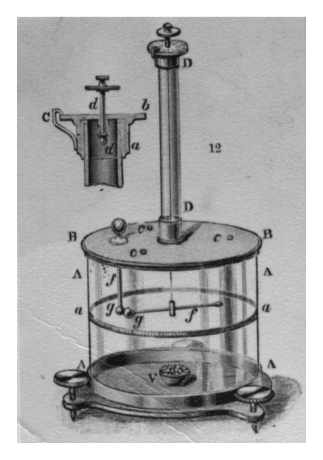
\includegraphics[scale=1.0]{resources/figura5.eps}
\caption{Balanza de torsión.}
\label{figura5}
\end{figure}

\item \textbf{¿Cuál cree que es mejor método para demostrar la Ley de
\emph{Coulomb}, la de la actual práctica o el de la balanza de torsión?
Explique su respuesta.}

Dadas las circunstancias, no podemos dar una opinión concisa debido a que no
pudimos experimentar de manera presencial los experimentos mencionados, y solo
contamos con el simulador para poder obtener los resultados.
\end{enumerate}

\end{document}

